%analyse + méthodo
Nous avons choisi de réaliser notre TER avec la méthode Agile car elle est utilisée en entreprise et elle permet d'avoir un projet fonctionnel à chaque fin de sprint.
Nous avons commencé le projet par l'analyse des outils et de l'existant, le langage Logo et des dérivés, ainsi que par réalisé un aperçu avec OpenProject (cf. 2.1) pour évaluer combien de sprint nous pourrions faire, en comptant le fait que nous avions des cours en même temps, des examens, la semaine de révisions,...\\
\begin{figure}[h]
\caption{\label{planning} Planning OpenProject}
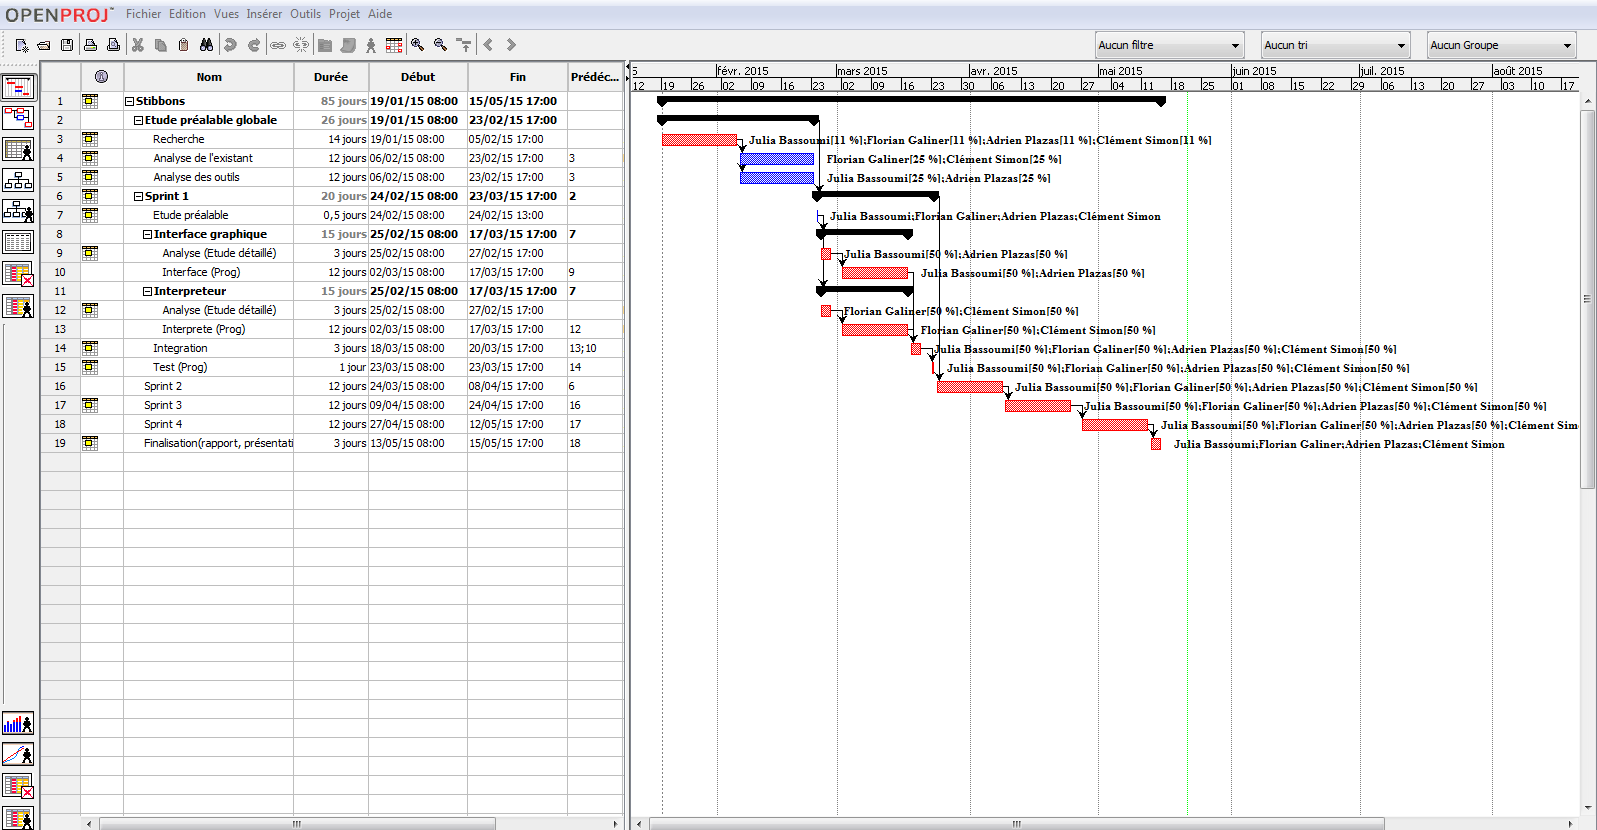
\includegraphics[scale=0.35]{doc/gestionProjet/planning.PNG}
\end{figure}
Ensuite nous avons défini les fonctionnalités et fait notre premier backlog (cf. Table 2.1) .
Nous avons attribué une priorité à chaque tâche du backlog, selon nos idées et celles de notre tuteur. Nous avons dévellopé à la manière d'un développement interne en entreprise, il n'y avait de client externe, puisque nous avons proposé notre projet.
Nous avons ensuite rédigé des scénarios utilisateur.
Pour l'estimation des heures de chaque sprint, nous procédions avec des petits papiers, où pour chaque tâches, chacun de nous mettons son estimation maximale et minimale, puis nous en discutions. L'estimation correspond à la moyenne entre la plus haute de toutes et la plus petite.
Pour la réalisation, nous nous sommes séparé en deux groupes de deux : un groupe Modèle-Interface et un groupe Grammaire-Interprète.
A chaque sprint, chacun avait une ou plusieurs tâches à faire, parfois seul, parfois en collaboration.

{\tiny
\begin{longtable}[c]{|c|p{1.3cm}|c|p{3.5cm}|*{3}{c|}p{0.7cm}|}
\hline
\bf id & \bf Scénario utilisateur & \bf Priorité & \bf Tests & \bf Estimation & \bf Sprint & \bf Statut & \bf Temps réel \\
\hline
\endfirsthead
\hline
\bf id & \bf Scénario utilisateur & \bf Priorité & \bf Tests & \bf Estimation & \bf Sprint & \bf Statut & \bf Temps réel \\
\hline
\endhead
\hline
\caption{Backlog Initial (fin).} \label{bsp1}\\
\endlastfoot
\hline
\caption[]{Backlog Initial.}\\
\endfoot
1 & L'utilisateur écrit du code dans un éditeur & 200 &  &  &  &  &  \\
\hline
2 & L'utilisateur importe du code dans le logiciel & 1100 & Importer du code Stibbons depuis un fichier, vérifier que le code obtenu est bien identique à celui du fichier. & 4h & 1 & ? & 1h \\
\hline
3 & L'utilisateur visualise les rapports d'erreurs du code & 400 &  &  &  &  &  \\
\hline
4 & L'utilisateur visualise l'évolution du modèle & 1400 & Vérifier que l'interprétation d'instructions données fait bien évoluer comme prévu la tortue dans son environnement. & 24h & 1 & Fini & 70h \\
\hline
5 & L'utilisateur modifie la vitesse (pause, pas à pas, parallèle) & 700 &  &  &  &  &  \\
\hline
6 & Le «dieu-tortue» interprète le code de l'utilisateur & 1500 & Lancer l'interprétation pour~: repeat 4 { fd 1 rt 90 } (suivant syntaxe) ainsi que pour du code avec des erreurs~: repat 4 {...} par exemple ou repeat 4 { fd 1 rt } & 12h & 1 & Fini & 32h \\
\hline
7 & L'utilisateur crée une nouvelle tortue (avec un code) & 600 & Lancer l'interprétation pour~: create-turtle {} et observer une nouvelle tortue apparaître dans l'interface graphique. & 7,5h & 2 &  &  \\
\hline
8 & Les tortues s'exécutent en parallèles & 1200 & Lancer l'interprétation pour deux tortues d'un bout de code et observer l'exécution parallèle via des écritures dans le terminal (Je suis tortue 1 et Je
suis tortue 2 par exemple) & 42,5h & 2 & & \\
\hline
9 & Les tortues communiquent directement entre elles & 900 &  &  &  &  &  \\
\hline
10 & Une tortue se déplace dans l'environnement & 1300 & Ecriture d'instructions simples~: repeat 4 { fd 1 rt 90 } (suivant syntaxe) - Renvoi de la position de la tortue après chaque deplacement~: where\_am\_i(); (suivant syntaxe) & 16h & 1 & Fini & 24h \\
\hline
11 & Les tortues communiquent avec les zones de l'environnement & 1000 &  &  &  &  &  \\
\hline
12 & L'utilisateur exporte le code & 500 &  &  &  &  &  \\
\hline
13 & L'utilisateur exporte le modèle & 300 &  &  &  &  &  \\
\hline
14 & L'utilisateur ajoute une entrée & 100 &  &  &  &  &  \\
\hline
15 & L'utilisateur remet à zéro l'environnement & 800 &  &  &  &  &  \\
\hline
16 & L'utilisateur utilise des variables dans le code & 1275 & Ecrire a = 90 fd a et observer la tortue qui avance. & 12h & 2 &  &  \\
\hline
17 & L'utilisateur définit des fonctions personnalisées dans le code & 1250 & Ecrire function f () { fd 90 } f () et observer la tortue qui avance. & 23,5h & 2 & &  \\
\hline
18 & Les tortues communiquent via l'environnement & 950 &  &  &  &  &  \\
\hline
19 & L'utilisateur utilise des conditionnelles & 550 & Ecrire if(false) { fd 90 } et observer que la tortue ne bouge pas. Refaire le même test avec if(true) et observer que la tortue bouge. & 3,5h & 2 &  &  \\
\hline
20 & L'utilisateur utilise des boucles & 575 & Ecrire pd repeat 4 { fd 40 rt 90 } et observer que la tortue dessine un carré. & 7h & 2 &  &  \\
\hline
\end{longtable}}
